%\documentclass[a4paper]{article}
\documentclass[preprint]{elsarticle}
%\usepackage[affil-it]{authblk}
%\setcounter{Maxaffil}{30}
\usepackage{footmisc}
%\usepackage{fnpct}
\makeatletter
\let\@fnsymbol\@alph
\makeatother
\usepackage[english]{babel}
\usepackage[utf8]{inputenc}
\usepackage{fancyhdr}
\setlength{\headheight}{100.0pt}
\usepackage{amsmath}
\usepackage{amssymb}
\usepackage{upgreek}
\usepackage{graphicx}
\usepackage{endnotes}
\usepackage{float}
\usepackage{caption}
\usepackage{subcaption}
\usepackage[colorinlistoftodos]{todonotes}
\usepackage{url}
\usepackage{lineno}
\usepackage{appendix}
\usepackage[colorlinks]{hyperref}
\usepackage{draftwatermark}
\SetWatermarkText{IDR HF v0.0}
\SetWatermarkScale{4}
\AtBeginDocument{%
  \hypersetup{%
    linkcolor=red,%
    citecolor=green,%
    urlcolor=cyan,%
  }%
}%

% Define the margins explicitly
\usepackage{geometry}
\geometry{
  pdftex=true,
  margin=30mm,
  bottom=30mm,
  top=30mm
  }


% Margins
%\topmargin=-0.45in
%\evensidemargin=0.0in
%\oddsidemargin=0.0in
%\textwidth=6.5in
%\textheight=10.0in
%\headsep=0.25in
%New definitions
\newcommand{\qgsp}{{\sc qgsp\_bert}}
\newcommand{\ftfp}{{\sc ftfp\_bert}}
\newcommand{\qbbc}{{\sc qbbc}}
\newcommand{\ecal}{Si-W ECAL}
\newcommand{\ecalp}{\ecal\ physics prototype}
\newcommand{\tfa}{track-finding algorithm}
\newcommand{\ep}{$\varepsilon$ parameter}
\newcommand{\gu}{${\rm g.u.}$ }
\newcommand{\geantfour}{{\sc geant4}}
\newenvironment{bottompar}{\par\vspace*{\fill}}{\clearpage}
\linenumbers



%\DefineFNsymbols*{asterisks}{*{$\dagger$}{$\ddagger$}{$\mathchar "278$}{$\mathchar "27B$}{$\|$}{**}{$\dagger\dagger$}{$\ddagger\ddagger$}{$\mathchar"27C$}}
%\setfnsymbol{asterisks}
%\renewcommand{\thefootnote}{\fnsymbol{thanks}}


\usepackage{fancyhdr}
\fancypagestyle{pprintTitle}{%
%\fancypagestyle{plain}{%
%\lhead{} \chead{}\rhead{Draft CALICE Paper 028\\ Version2.4\\ Paper version 1.5}
%\lhead{} \chead{}\rhead{Draft CALICE Paper 028\\Version 2.6\\ \today}
\lhead{} \chead{}\rhead{ILD-NOTE-2019-XXX}
\lfoot{}\cfoot{}\rfoot{}
\renewcommand{\headrulewidth}{0.0pt}
}


%\pagestyle{fancy}
%\fancyhf{}
%\fancyhead[LE,RO]{Overleaf}
%\fancyhead[RE,LO]{Guides and tutorials}
%\fancyfoot[CE,CO]{\leftmark}
%\fancyfoot[LE,RO]{\thepage}

%\usepackage{manyfoot}
%\newcommand{\Afootnoterule}{}
%\SelectFootnoteRule{A}[\noindent\footnotesize Custom Footnotes:\vspace{2mm}]
%\DeclareNewFootnote{A}[roman]



%\fancypagestyle{plain}{%
 % \renewcommand{\headrulewidth}{0pt}%
 % \fancyhf{}%
 %\fancyhead[R]{Draft CALICE Paper 028\\
 %        Version 2.4\\
 %          \today\\}%
%} 

%\title{\bf Tracks of hadronic showers in the \ecalp }
%\title{\bf Tracks of hadronic showers in the \ecalp \\
%\bigskip\bigskip\bigskip
%CALICE Collaboration}



%



%\include{AuthorListPaper028Tex}

%\author{R. P\"oschl }
%\include{AuthorListPaper028Tex}

%\date{\today}

\begin{document}
%\input{AuthorListPaper028Tex}

\begin{frontmatter}

%\title{ {\LARGE\bf A precise determination of top quark electro-weak couplings at the ILC operating at $\roots=500\,\GeV$}}
\title{\LARGE\bf Heavy Flavour Benchmarks of ILD}

%\include{auth-pap028}


\begin{abstract}
An overview of the performance of the ILD detector in its version Large and Small as relevant for the IDR is given 

\end{abstract}


\end{frontmatter}


%\begin{titlepage}
%\begin{flushright}
%Draft CALICE Paper 028\\
%          Version 2.4\\
%           \today\\
%\end{flushright}
%\maketitle 
%\bigskip\bigskip\bigskip\bigskip\bigskip\bigskip

%\begin{center}
%\huge \bf 
%Tracks of hadronic showers in the \ecalp

%\end{center}\bigskip\bigskip 
%\begin{center}{
%{\LARGE The CALICE Collaboration}

%\footnote{Corresponding authors: \\ Roman P\"oschl: {\tt poeschl@lal.in2p3.fr}, Sviatoslav Bilokin: {\tt bilokin@lal.in2p3.fr}}}
%\end{center}\bigskip\bigskip
%\bigskip%\begin{center}{\large  Abstract}\end{center}



%\begin{bottompar}
%\begin{center}
%\vspace{2cm}
%{\sl This note contains preliminary CALICE results, and is for the use
%of members of the CALICE Collaboration and others to whom permission
%has been given.}
%\end{center}
%\end{bottompar}
%\end{titlepage}


%\thispagestyle(fancy)
%\newpage
\tableofcontents



%------------------Introduction---------------------%
\section{Introduction}

It has been shown in recent publications that heavy quarks may be important messengers of new physics. High precision $e^+e^-$ collisions with polarised beams around the TeV scale are ideally suited to detect new physics effects. The detection of the onset of new physics require however a superb detector performance in terms of flavor tagging including the event by event determination of the charge of the final state jets. The charge determination happens mainly by a combination of the determination of the summed charge of tracks pointing to a secondary vertex or by the identification of the charge of a final state Kaon. This is turn requires a successful particle identification by the detector. 
Therefore processes with heavy quark final states, i.e. $e^+e^-\rightarrow b\bar{b}$  and $e^+e^-\rightarrow t\bar{t}$ are highly relevant for the benchmarking of the detector performance. In short one can test the following detector capacities. 

\begin{itemize}
\item Track finding efficiency 
\item Stringent test of (secondary) vertexing
\item Particle ID
\item In case of $e^+e^-\rightarrow t\bar{t}$  leptonic and semi-leptonic decays of the top-quark pair provide an important additional handle for the accurate measurement of the final state. The analysis presented in this note focuses on the semi-leptonic decay mode of the top-quark pair. 
\end{itemize}
%General introduction
The analyses presented in this note start out from the PhD thesis of Sviatoslav Bilokin that are based on the DBD samples and software versions. This work has in part been published as arxiv:1709.xxxx. The analyses are ported to the large and small detector models and are carried out with the software version that is relevant for the IDR of ILD. For the process $e^+e^-\rightarrow b\bar{b}$ an analysis at $\sqrt{s}=500$\,GeV is presented instead of $\sqrt{s}=250$\,GeV as in Refs.. The results also benefit from a refined analysis strategy for the ILD paper that is under review in ILD. 

\section{Methods, tools and Monte Carlo samples}

For the event reconstruction we use the \texttt{ILCSoft} version \texttt{v02-00-02} 
We use the following methods
\begin{itemize}

\item `Core tools'
  \begin{itemize}
  \item We use the \texttt{ValenciaVertex} jet algorithm implemented in \texttt{LCFIPlus} that provides the rejection of $\gamma\gamma$ background. In this algorithm the distance between two objects is calculated as  
  \begin{equation}
d_{ij} = 2 \min(E^{2\beta}_{i}, E^{2\beta}_{j}) (1-\cos \theta_{ij})/R^2
  \end{equation}
The distance of a particle $i$ to the beam is calculated according to.
  \begin{equation}
d_{iB} = E^{2\beta} \sin^{2\gamma}\theta_{iB}
  \end{equation}

  The jet algorithm is run with the following settings: $\alpha=\beta=\gamma=1$, $R=1.4$ 
  \item We use the \texttt{LeptonFinder} in case of semi-leptonic $e^+e^-\rightarrow t\bar{t}$ events
  \item For the vertex finding we use the \texttt{LCFIPlus} version v.xxxx. QUESTION: DO WE USE THE REPROCESSED SAMPLES BY RYO?
  \end{itemize}
%\item Using TPC dE/dx to identify Kaons issue of the B-Meson decays (Processors????)

\item Tools developed for the study
  \begin{itemize}
  \item The \texttt{VertexRestorer} Processor identifies tracks that have not been associated to secondary vertices from B-Meson decays but belongs to this decay according to the Monte Carlo Truth information. It then recovers the `lost' tracks by means of the impact parameters $d_0$ (transversal) and $z_0$ (longitundinal).     
In this present note the recovery uses only the impact parameter $d_0$ since the algorithms needs to be adapted for the vertex smearing present in the simulation for the IDR. 
%Analysis of tracks associated to the secondary vertex (LCFIPlus v.xxxx and navigations through reconstructed particle list using LCRelations)
%    \begin{itemize}
%    \item Purpose: Identify and add tracks that have not been associated in Standard Reco (VertexRecoveryProcessort)
%    \end{itemize}
\item The \texttt{ParticleTagger} Processor identifies the Kaons by means of the dE/dx measured in the TPC of ILD. It selects a strip in the dE/dx-momentum plane with a high kaon concentration. The efficiency and the purity of the Kaon selection vary as a function of the width of this strip. 
\item The \texttt{QQbarAnalysis} Processor calculates the jet charge and the polar angle of the bottom and top quark pair, respectively. It contains separate  methods for the bottom and top quark pair analysis.
 
\item The \texttt{TrashRecoProcessor} enables comparisons between reconstructed and generated quantities. 

\item The described tools are available under \url{https://github.com/QQbarAnalysis}. This repository contains also a set of macros necessary for the final steps of the analysis.

\end{itemize}



\item Quark charge measurement and corrections for miscalculations

  \begin{itemize}
  \item Probabilities on double charge measurements for $t\bar{t}$ and $b\bar{b}$ has been examined.
  \item Calculations scheme is shown below.
    \begin{align}
      \left.
      \begin{aligned}
        N_{acc} &= Np^2 + Nq^2\\
        N_{rej} &= 2Npq\\
        1 &= p + q
      \end{aligned}
      \right\}
      \quad N_{corr} = N_{acc} \cdot \frac{p^2}{p^2 + q^2}
    \end{align}
  \label{eq:pq-meth}
  \item where $N$ is total number of events, $N_{acc}$ and $N_{rej}$ are number of events that were accepted and rejected, respectively. $p$ and $q$ values represents probabilities of events being accepted and rejected. Solving this equation will give us back both p and q, thus improving our results on $A_{fb}$.
  \item the correction has been applied to the $b\bar{b}$ studies while not in $t\bar{t}$. Selection scheme in $t\bar{t}$ is much more complicated than that for $b\bar{b}$ thus applying the correction will reduce the efficiency with little effect.
%  \item Plots. $t\bar{t}$: Figure.~\ref{fig_eff_purity}, $b\bar{b}$: Figure.~\ref{fig_eff_purity}.
       
  \end{itemize}
  
 \end{itemize}

%\begin{equation}
%	\vec{x} = (x,y,z)=\left
%\{
%\begin{array}{c}
%x= 0 .. 17 \\ 
%y=0 .. 17 \\
%z = 0 .. 29,
%\end{array}
%\right.
%\end{equation}



%|||||||||||||||||||Description of a dataset||||||||||||||||||||%



%\begin{figure}[H]
%\centering
%\includegraphics[width=0.95\textwidth]{new_beamline.png}
%\caption{\label{fig:fnal-beamline} \sl Plan view of the beam line at FNAL. Distances (not to scale) are in mm.}
%\end{figure}

\subsection{ Monte Carlo samples and Event processing}
For this benchmark study only processes with {\em left-handed} electron polarisation and {\em right-handed} positron polarisation have been studied so far. The final states resulting from this configuration are more demanding for the detector performance in terms of the control of migration effects. 

More precisely the results presented in this note are based on the following samples:
\begin{itemize}
\item $e^+e^-\rightarrow t\bar{t}$: 
\begin{itemize}
\item  $yyxye\nu$: \url{https://ild.ngt.ndu.ac.jp/elog/opt-data/?GenProcessID=108670}\\
This sample contains the final state resulting from the $W\rightarrow e\nu$ decay.
The generated cross section is $116.9\,{\rm fb}$ and the total integrated luminosity is about $2200\,{\rm fb^{-1}}$. CHECK EVENT NUMBERS!!!
\item  $yyxyl\nu$: \url{https://ild.ngt.ndu.ac.jp/elog/opt-data/?GenProcessID=108675}. \\  
This sample contains the final state resulting from the $W\rightarrow \ell\nu$ decay with $\ell=\mu,\tau$.
The generated cross section is $213.25\,{\rm fb}$ and the total integrated luminosity is about $2100\,{\rm fb^{-1}}$. CHECK EVENT NUMBERS.
For the analysis presented here the final state with $\ell=\tau$ has been discarded.
\end{itemize}
\item  $e^+e^-\rightarrow b\bar{b}$:  \url{https://ild.ngt.ndu.ac.jp/elog/opt-data/?GenProcessID=250114}
The generated cross section is $32470\,{\rm fb}$ and the total integrated luminosity is about $46\,{\rm fb^{-1}}$
\end{itemize}

In both cases the samples available for small and large detectors are available and comparisons will be presented where appropriate. 

\section{Efficiencies and Control plots }


\begin{figure}
\centering
\includegraphics[width=0.45\textwidth]{figures_Methods/bjet_v2.eps}
\caption{\label{fig:control-bjet-mom} \sl Momentum of the b-jet with cheated identification for  $e^+e^-\rightarrow b\bar{b}$ and $e^+e^-\rightarrow t\bar{t}$ processes.}
\end{figure}



The Figs.~\ref{fig:vtx-recov-bbbar} and~\ref{fig:vtx-recov-ttbar} show the missed tracks before and after vertex recovery for the $e^+e^-\rightarrow b\bar{b}$ and $e^+e^-\rightarrow t\bar{t}$  analyses, respectively. Both figures suggest a systematic improvement in the assignment of secondary vertices. This improvement is quantified in Figs.~\ref{vr_and_bquarkpurity_bbbar} and~\ref{vr_and_bquarkpurity_ttbar} where the purity of the b-charge reconstruction is shown as a function of 
the $b-tag$ valaue,  the reconstructed $b$-momentum $|p_{had}|$ the number of reconstructed tracks assigned to a secondary vertex $N_{rec}$ and finally the polar angle of the $b$-hadron. here denoted as $|\cos \theta|$. The improvemt is is larger for the process $e^+e^-\rightarrow t\bar{t}$  than for $e^+e^-\rightarrow b\bar{b}$. Qualitatively this is expected since the tracks produced in the decay of the b-hadron are softer in case of top-pair production. In case of $e^+e^-\rightarrow t\bar{t}$ the improvemnt is 10\% over a large range in $|\cos \theta|$ and mainly driven by three to five prong decays.  Both results will further improve once the vertex recovery takes also the the impact parameter $z_0$ into account. All results shown so far in this section have been obtained for the large detector model. The conclusions for the small detector model are similar. 

\begin{figure}
\centering
\includegraphics[width=0.45\textwidth]{figures_Methods/beforeVR_bbbar_l5.eps}
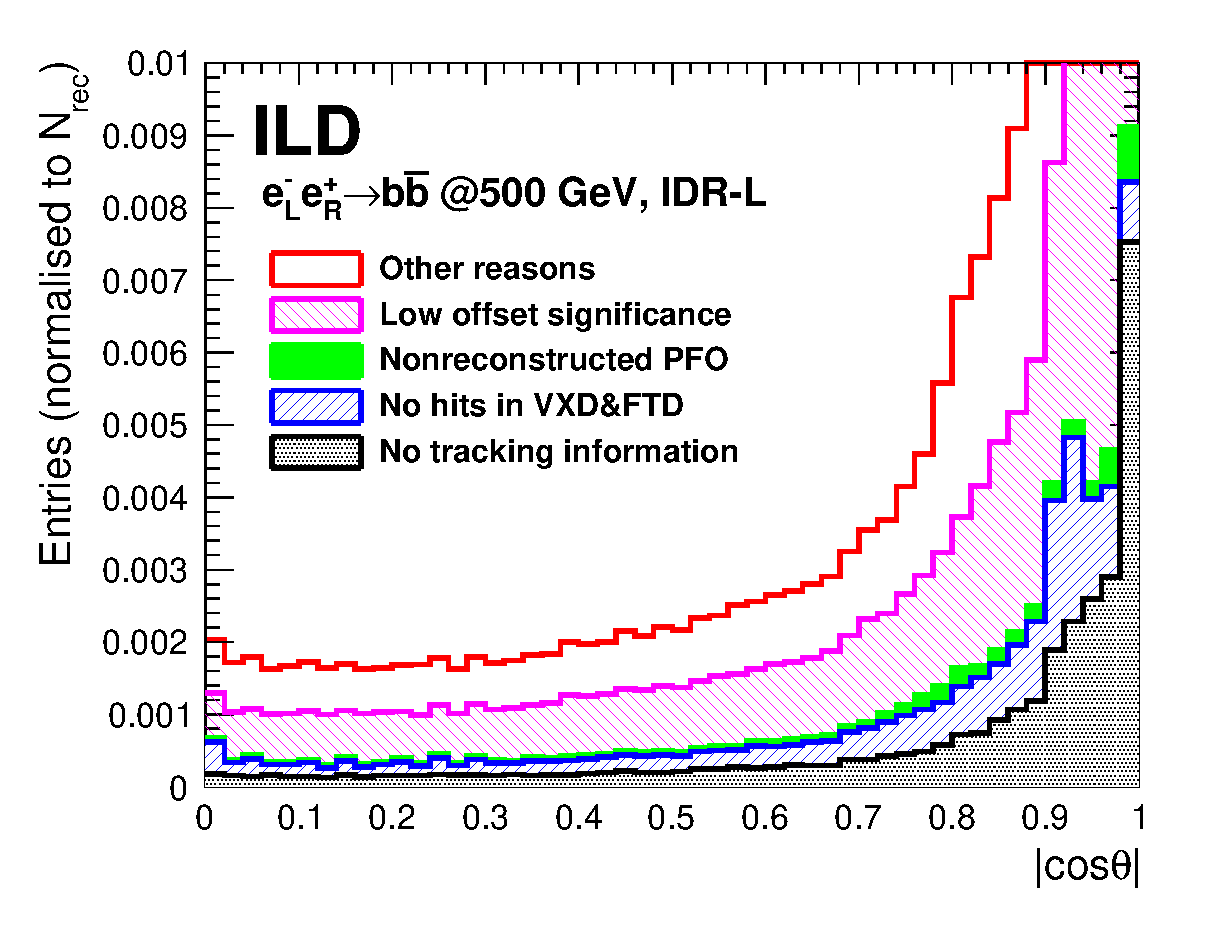
\includegraphics[width=0.45\textwidth]{figures_Methods/afterVR_bbbar_l5.eps}
\caption{\label{fig:vtx-recov-bbbar} \sl Vertex recovery in case of the  $e^+e^-\rightarrow b\bar{b}$ process.}
\end{figure}

\begin{figure}
\centering
\includegraphics[width=0.45\textwidth]{figures_Methods/beforeVR_ttbar.png}
\includegraphics[width=0.45\textwidth]{figures_Methods/afterVR_ttbar.png}
\caption{\label{fig:vtx-recov-ttbar} \sl Vertex recovery in case of the  $e^+e^-\rightarrow t\bar{t}$ process.}
\end{figure}


\begin{figure}
\centering
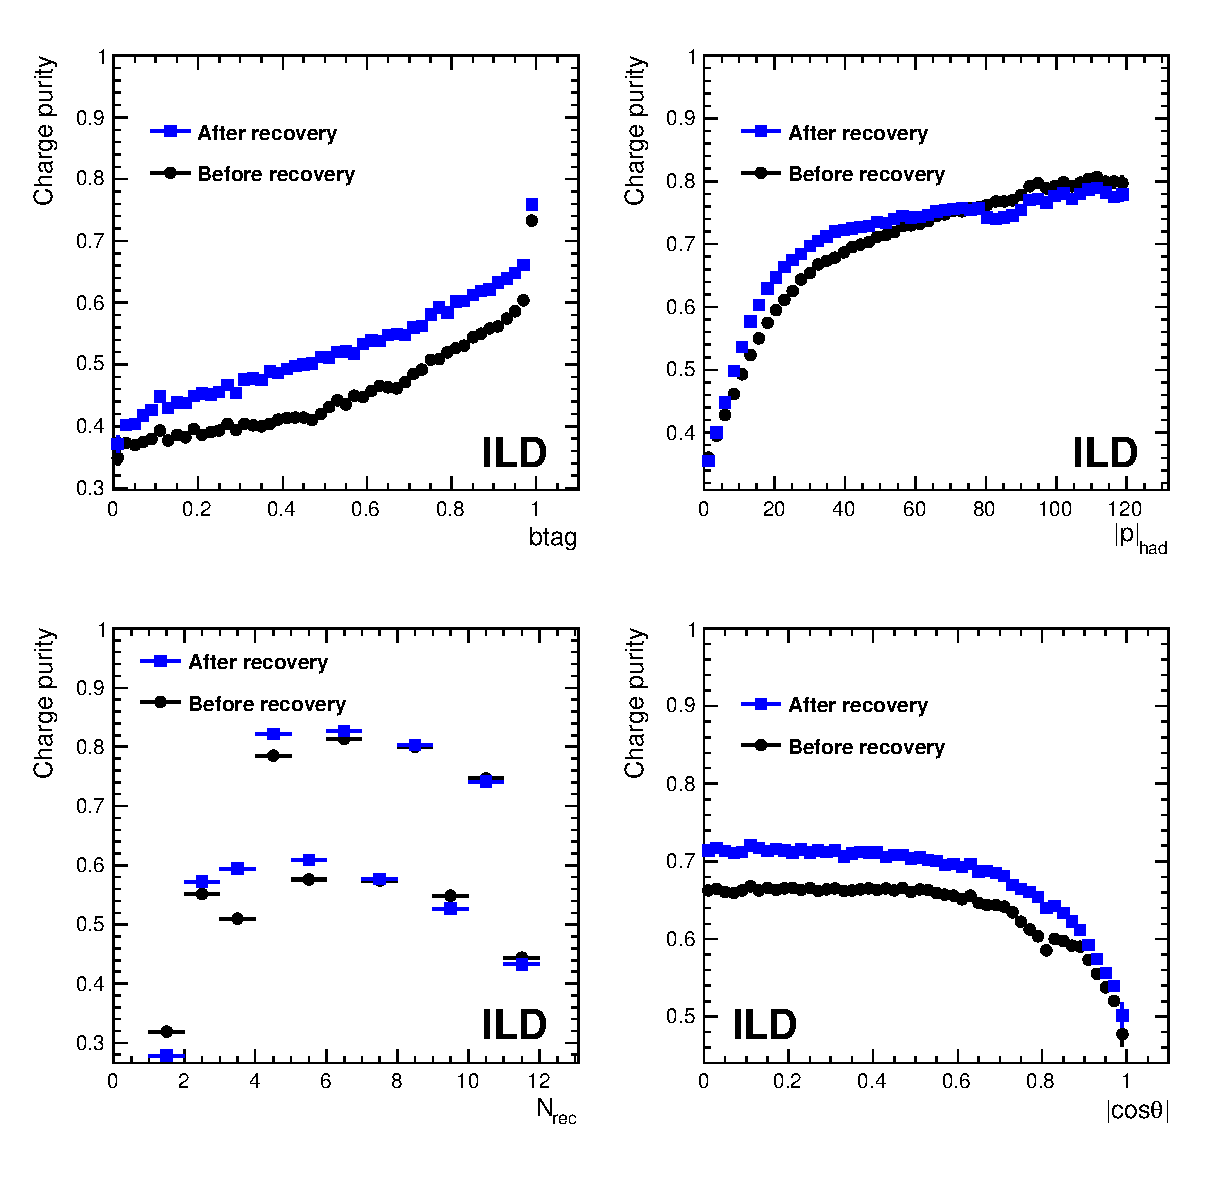
\includegraphics[width=0.8\textwidth]{figures_Methods/b_purity_VR_ttbar_l5.eps}
%\includegraphics[width=0.45\textwidth]{figures_Methods/afterVR_ttbar.png}
\caption{\label{vr_and_bquarkpurity_bbbar} \sl Purity before and after vertex recovery in case of the  $e^+e^-\rightarrow b\bar{b}$ process for different observables.}
\end{figure}

\begin{figure}
\centering
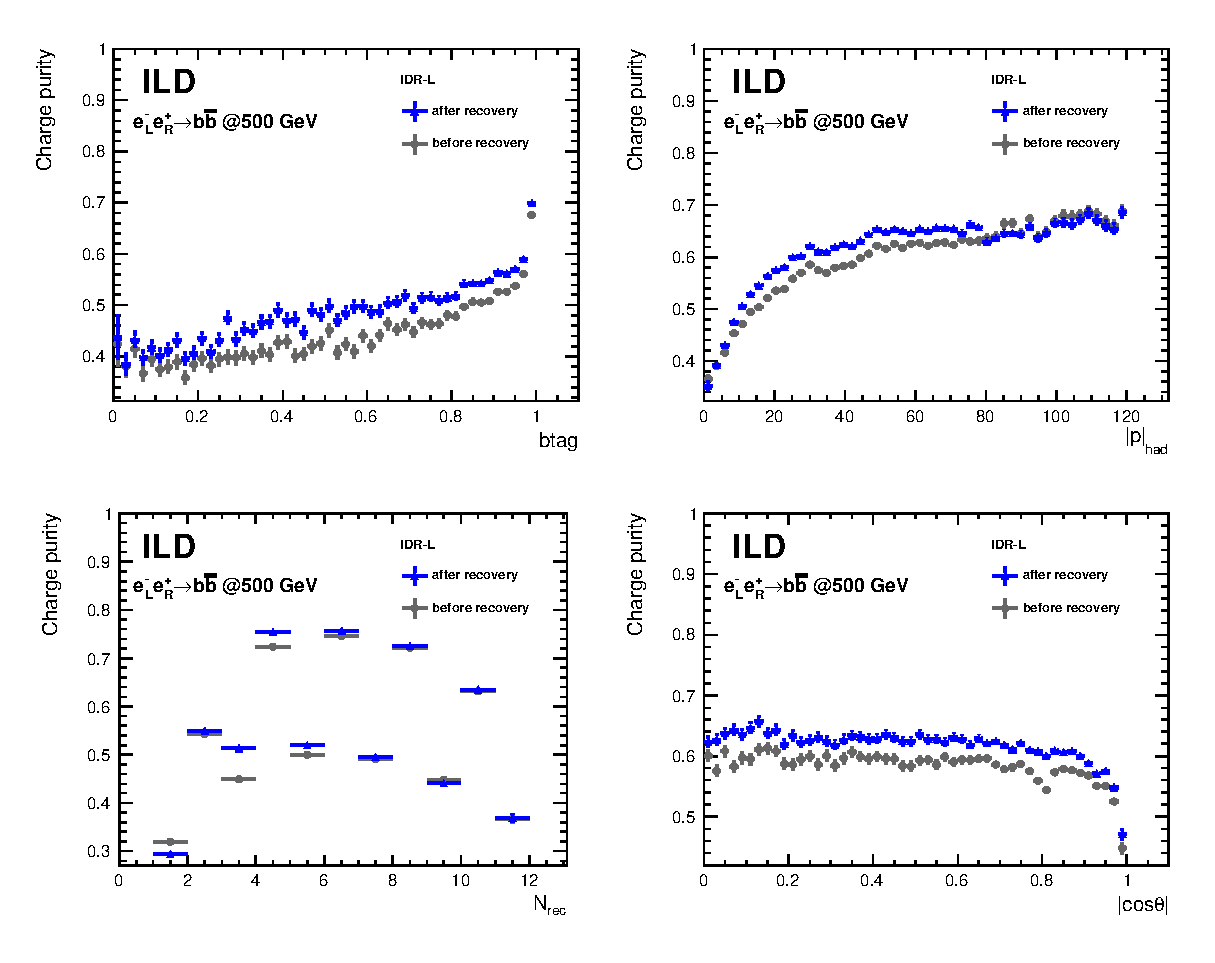
\includegraphics[width=0.8\textwidth]{figures_Methods/b_purity_VR_bbbar_l5.eps}
%\includegraphics[width=0.45\textwidth]{figures_Methods/afterVR_ttbar.png}
\caption{\label{vr_and_bquarkpurity_ttbar} \sl Purity before and after vertex recovery in case of the  $e^+e^-\rightarrow t\bar{t}$ process for different observables.}
\end{figure}


The lower right panels of Figs.~\ref{vr_and_bquarkpurity_bbbar} and~\ref{vr_and_bquarkpurity_ttbar} show a drop in purity for large values of $|\cos \theta|$. This is compatible with the drop in acceptance that is shown in Fig.~\ref{fig_acceptance_bb} for the case $e^+e^-\rightarrow b\bar{b}$ as a function of the plolar angle of the reconstructed $b$-jet $|\cos \theta_b|$. Within statistical errors the results are the same for the large and the small detector model. However, towards large values of   
$|\cos \theta_b|$ the large detector performs systematically better than the small detector.

A component that distinguishes the ILD Detector from other proposals for $e^+e^-$ colliders is the TPC as the central tracking system. Beside the precise momentum measurement the dE/dx measurement in the gaseous medium allows for a particle identification. Since around 80\% of B-Mesons (neutral or charged) contain a charged Kaon among their decay products the particle ID can support greatly the charge determination of the $b$-quark. The Fig.~\ref{fig_dEdx_1} displays the normalised dE/dx spectrum for different particles in different momentum ranges for the large and the small detector model. In both cases there is a clear separation of Kaons from pions. The latter are however much more abundant. There is only a small population of protons. Figure~\ref{fig_dEdx_2} shows the dE/dx spectra for the two processes under study. Finally the Fig.~\ref{kaonID_effpurity} shows the variation of the purity as as a function of the Kaon selection efficiency.



%\begin{itemize}

%\item Common
%\begin{itemize}
%\item it might be good to produce a plot of the b-momentum in the lab frame to point out the differences between the two final states.
%\item Plots before and after vertex recovery (at least initially b and t analysis, large detector is enough unless striking difference). DONE
%\item Increase of purity by vtx recovery (b and t analysis, large detector is enough unless striking difference). DONE
%\item Detector acceptance (here maybe large and small) Slide 11 by Adrian DONE.
%\item dE/dx including `Jenny's' Plot, it's maybe sufficient to use the plots produced by Adrian. DONE
%\end{itemize}


%\begin{figure*}[!ht]
%  \centering
%  \begin{tabular}{l}
%    \begin{subfigure}{\textwidth}
%      \centering
%      \begin{tabular}{ll}
%        \centering
%        \includegraphics[width=0.4\textwidth]{figures_Methods/beforeVR_ttbar.png} & \includegraphics[width=0.4\textwidth]{figures_Methods/afterVR_ttbar.png}\\
%      \end{tabular}
%      \caption{ Left, lost tracks in reconstructed vertexes before recovery. Right, lost tracks in reconstructed vertexes after recovery.}
%      \label{vr_and_bquarkpurity_ttbar:a}
%    \end{subfigure} \\
%    \begin{subfigure}{\textwidth}
%      \centering
%      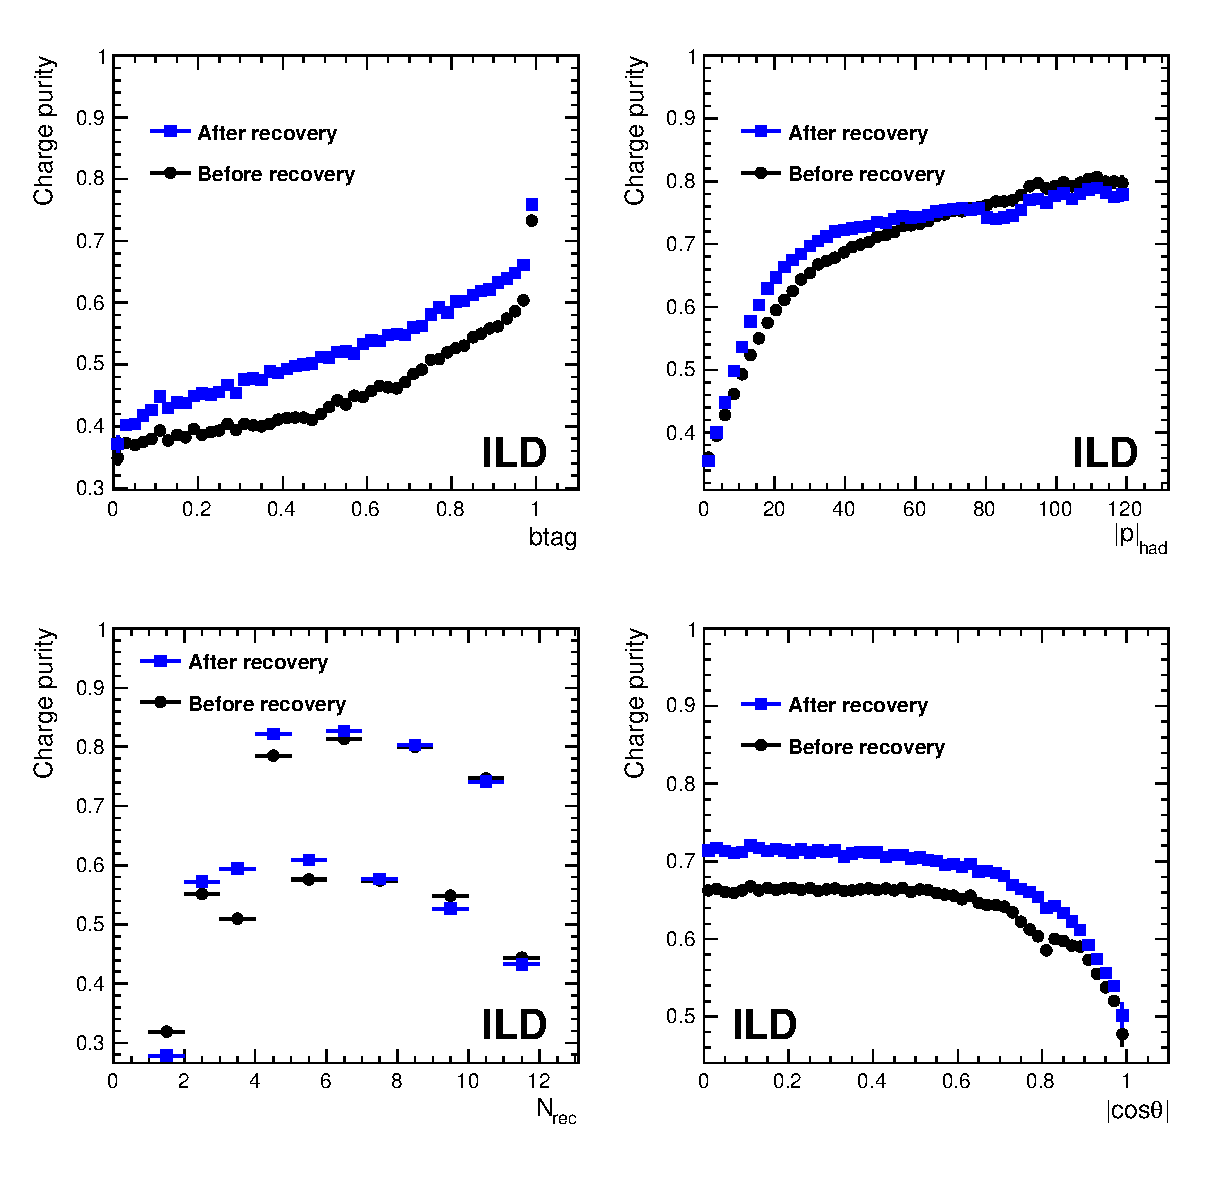
\includegraphics[width=0.8\textwidth]{figures_Methods/b_purity_VR_ttbar_l5.eps}
%      \caption{Lower plot, B-quark charge purity in single jets as a function of different kinematic variables, after and before recovery.}
%      \label{vr_and_bquarkpurity_ttbar:b}
%    \end{subfigure}%
%  \end{tabular}
%  \caption{$t\bar{t}$.  }
%  \label{vr_and_bquarkpurity_ttbar}
%\end{figure*}


%\begin{figure*}[!ht]
%  \centering
%  \begin{tabular}{l}
%    \begin{subfigure}{\textwidth}
%      \centering
%      \begin{tabular}{ll}
%        \centering
%        \includegraphics[width=0.4\textwidth]{figures_Methods/beforeVR_bbbar_l5.eps} & 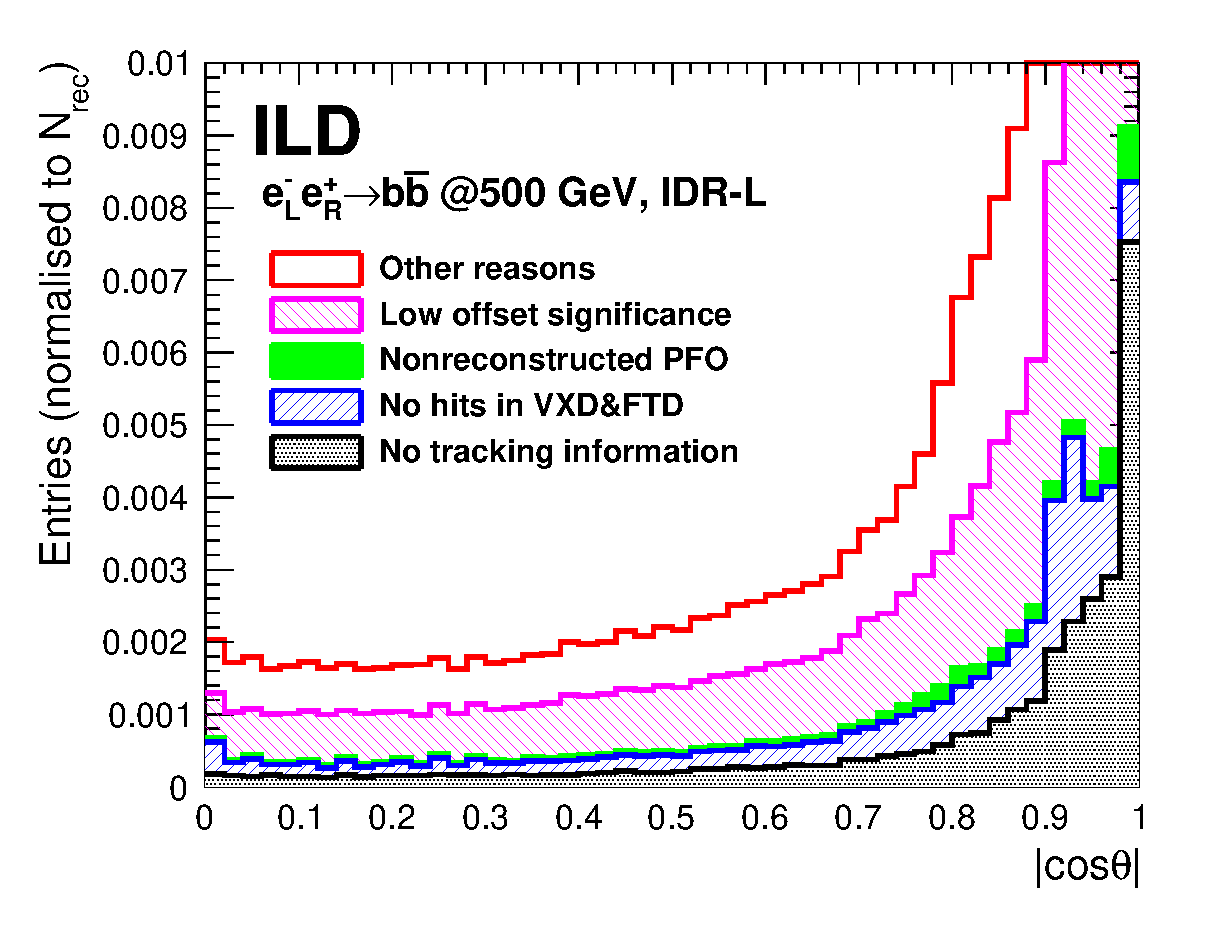
\includegraphics[width=0.4\textwidth]{figures_Methods/afterVR_bbbar_l5.eps}\\
%      \end{tabular}
%      \caption{ Left, lost tracks in reconstructed vertexes before recovery. Right, lost tracks in reconstructed vertexes after recovery.}
%      \label{vr_and_bquarkpurity_bbbar:a}
%    \end{subfigure} \\
%    \begin{subfigure}{\textwidth}
%      \centering
%      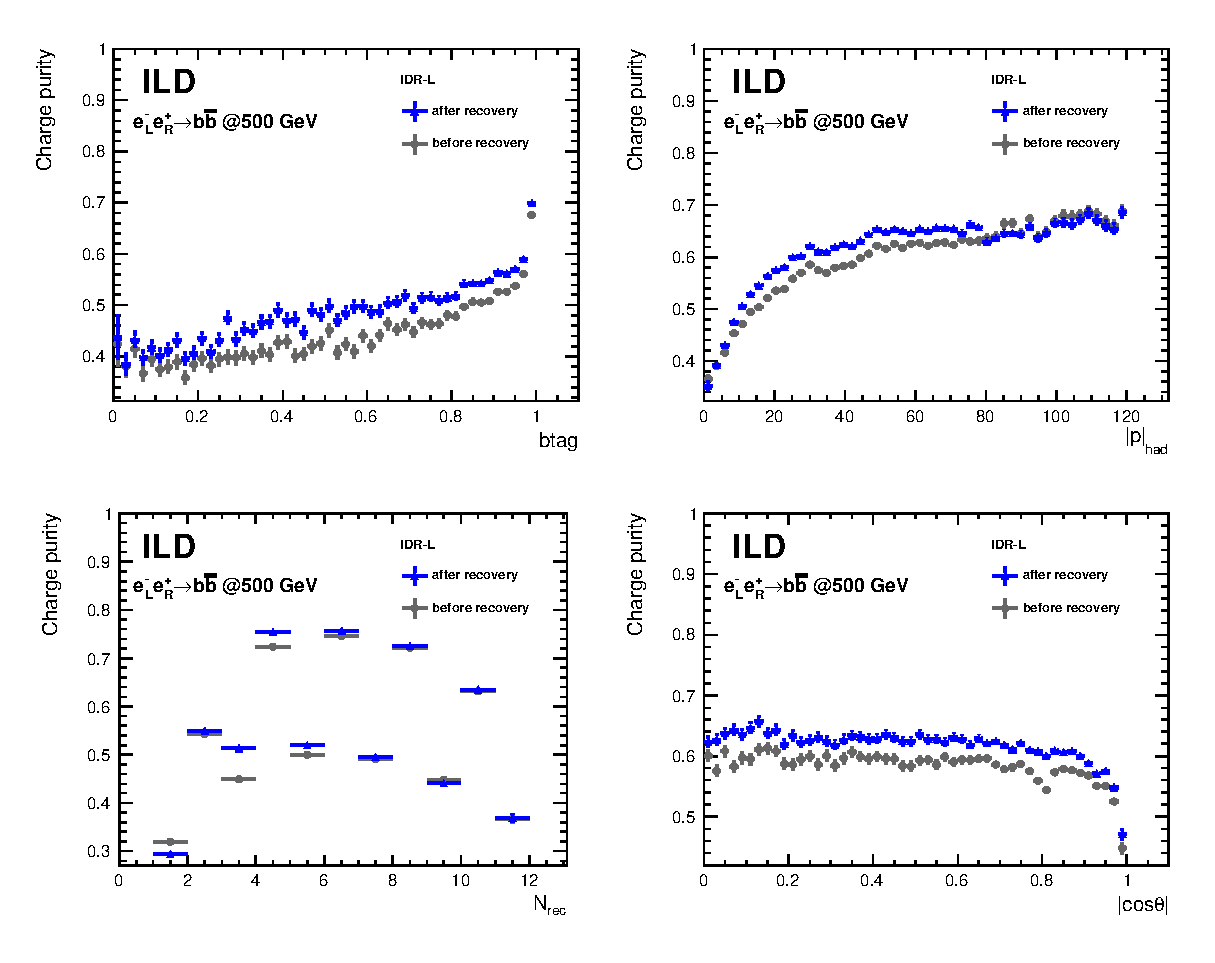
\includegraphics[width=0.8\textwidth]{figures_Methods/b_purity_VR_bbbar_l5.eps}
%      \caption{Lower plot, B-quark charge purity in single jets as a function of different kinematic variables, after and before recovery.}
%     \label{vr_and_bquarkpurity_bbbar:b}
%    \end{subfigure}%
%  \end{tabular}
%  \caption{$b\bar{b}$.  }
%  \label{vr_and_bquarkpurity_bbbar}
%\end{figure*}

\begin{figure}[h!]
\centering
  \includegraphics[width=0.6\textwidth]{figures_BBbar/acceptance_2models_v2.eps} 
\caption{Detector acceptance distribution for b-tagged jets. WHY IS THERE A PLATEAU AT 0.32? TAB~\ref{table_eff_bbbar} REPORTS AN OVERALL EFFICIENCY OF 64 - 65\%\% }
\label{fig_acceptance_bb}
\end{figure}

\begin{figure}[h!]
\centering
\begin{tabular}{ll}
  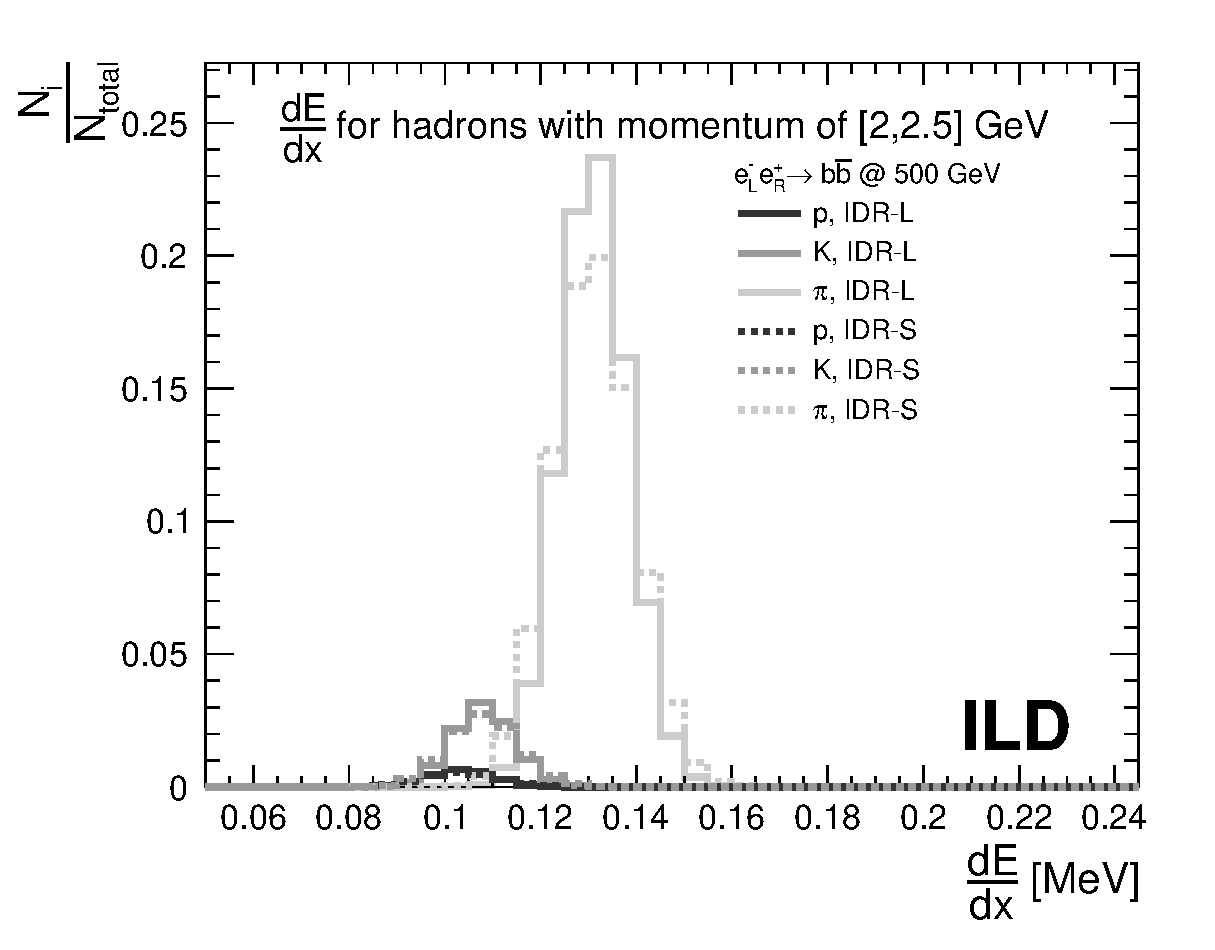
\includegraphics[width=0.5\textwidth]{figures_Methods/separation_had_2GeV_models_v2.eps} & 
  \includegraphics[width=0.5\textwidth]{figures_Methods/separation_had_5GeV_models_v2.eps} \\ 
  \includegraphics[width=0.5\textwidth]{figures_Methods/separation_had_10GeV_models_v2.eps} & 
  \includegraphics[width=0.5\textwidth]{figures_Methods/separation_had_10GeV_models_v2.eps} 	
\end{tabular}
\caption{Projection of dE/dx for several momentum ranges. Comparison of hadron separation performance by different detector models in $b\bar{b}$ final states.}
\label{fig_dEdx_1}
\end{figure}

\begin{figure}[h!]
\centering
\begin{tabular}{ll}
  \includegraphics[width=0.5\textwidth]{figures_Methods/separation_had_2GeV_bbbar_vs_ttbar_v2.eps} & 
  \includegraphics[width=0.5\textwidth]{figures_Methods/separation_had_5GeV_bbbar_vs_ttbar_v2.eps} \\ 
  \includegraphics[width=0.5\textwidth]{figures_Methods/separation_had_10GeV_bbbar_vs_ttbar_v2.eps} & 
  \includegraphics[width=0.5\textwidth]{figures_Methods/separation_had_10GeV_bbbar_vs_ttbar_v2.eps} 	
\end{tabular}
\caption{Projection of dE/dx for several momentum ranges. Comparison of hadron separation performance by the large model for different topologies. }
\label{fig_dEdx_2}
\end{figure}

\begin{figure}[h!]
\centering
  \includegraphics[width=0.6\textwidth]{figures_Methods/kaonIDeff_v2.eps} 
\caption{QUESTION: ARE THE DIFFERENT VALUES OF PURITY AND EFFICIENCY DUE TO A VARIATION OF THE STRIP IN THE DE/DX-MOMENTUM PLANE?}
\label{kaonID_effpurity}
\end{figure}


\section{Analysis details  specific to bb analysis}

Table~\ref{table_eff_bbbar} shows the selection efficiencies for the $e_{L}^{-}e_{R}^{+}\rightarrow b\bar{b}$ analysis. The overall efficiency is with around 64\% to 65\% 
similar for both detector models. For the $b$-charge measurement opposite charges in opposite jets are required. The charges are either derived from the tracks pointing to the secondary vertex or from the Kaon charge or from a combination of both.  The efficiencies for the different methods are given in Tab.~\ref{table_charge_calc_bbbar}. The purity of the different methods is shown in Fig.~\ref{purity_bb} . In both cases there is no large difference between the two detector models although the large detector seem to perform slightly better for the double Kaon method.

%\begin{itemize}
%\item Table with selection efficiencies DONE
%\item Is there anything specific to the bb analysis given that bb is a subsystem of tt?
%\end{itemize}

\begin{table}[t]
  \begin{center}\renewcommand{\arraystretch}{1.6}
    \begin{tabular}{l|l|l|l|l|l|l} 
    \multicolumn{7}{c}{$e_{L}^{-}e_{R}^{+}\rightarrow b\bar{b}$ at 500 GeV }\\
      \hline
      \hline
       & \multicolumn{3}{c|}{IDR-L} & \multicolumn{3}{|c}{IDR-S}\\
       & Signal& B$_{q\bar{q}}$/S & B$_{rad. Z}$/S & Signal & B$_{q\bar{q}}$/S & B$_{rad. Z}$/S\\
      \hline
      Full sample   & 100.0\% & 1800.5\% & 359.1\% & 100.0\% & 1800.6\% & 359.0\% \\
      $b_{tag}(jet_{1})>0.9$ and $b_{tag}(jet_{2})>0.2$    & 70.2\% & 2.3\% & 147.7\%  & 69.9\% & 2.3\% & 149.0\% \\
      $m_{jet_{1}+jet_{2}}>200 GeV$    & 68.2\% & 1.4\% & 6.7\%  & 67.8\% & 1.2\% & 6.7\% \\
      $E_{photon}<100 GeV$    & 64.8\% & 1.3\% & 1.7\% & 64.3\% & 1.2\% & 1.6\% \\
      double jet-charge measurement    & 28.9\% & 1.0\% & 1.0\% & 27.9\% & 0.9\% & 1.0\% \\
      \hline
      \hline     
    \end{tabular}
 \end{center}
 \caption{Selection efficiency and B/S rejection for some bkg sources}
\label{table_eff_bbbar}
\end{table}


\begin{table}[t]
  \begin{center}\renewcommand{\arraystretch}{1.6}
    \begin{tabular}{l|l|l} 
    \multicolumn{3}{c}{$e_{L}^{-}e_{R}^{+}\rightarrow b\bar{b}$ at 500 GeV }\\
      \hline
      \hline
       & IDR-L & IDR-S\\
      \hline
      Vtx+Vtx   & 12.9\% & 12.8\% \\
      K+K    & 4.4\% & 4.0\% \\
      Vtx+K (diff. jets)    & 3.9\% & 3.7\% \\
      Vtx+K (same jet) & 7.7\% & 7.4\% \\
      \hline
      \hline     
    \end{tabular}
 \end{center}
 \caption{Final selection efficiency, after double jet-charge measurement}
 \label{table_charge_calc_bbbar}
\end{table}
    
\begin{figure}[h!]
\centering
  \includegraphics[width=0.8\textwidth]{figures_BBbar/purity_v2.eps} 
\caption{Purity of the different methods}
\label{purity_bb}
\end{figure}

\section{Analysis details specific to tt-analysis}

\begin{itemize}
\item Energy and polar angle spectrum of selected isolated lepton MISSING
\item Table with selection efficiencies MISSING OR BETTER INCOMPLETE
\item For the record we may add the observation by Amjad on the b/c tagging.
\end{itemize}



Figure~\ref{fig_eff_purity} shows the fraction of accepted events, see Eq.~\ref{eq:pq-meth}  for different methods used to distinguish the top from the anti-top.  
\begin{figure}[h!]
    \centering
    \begin{tabular}{ll}
      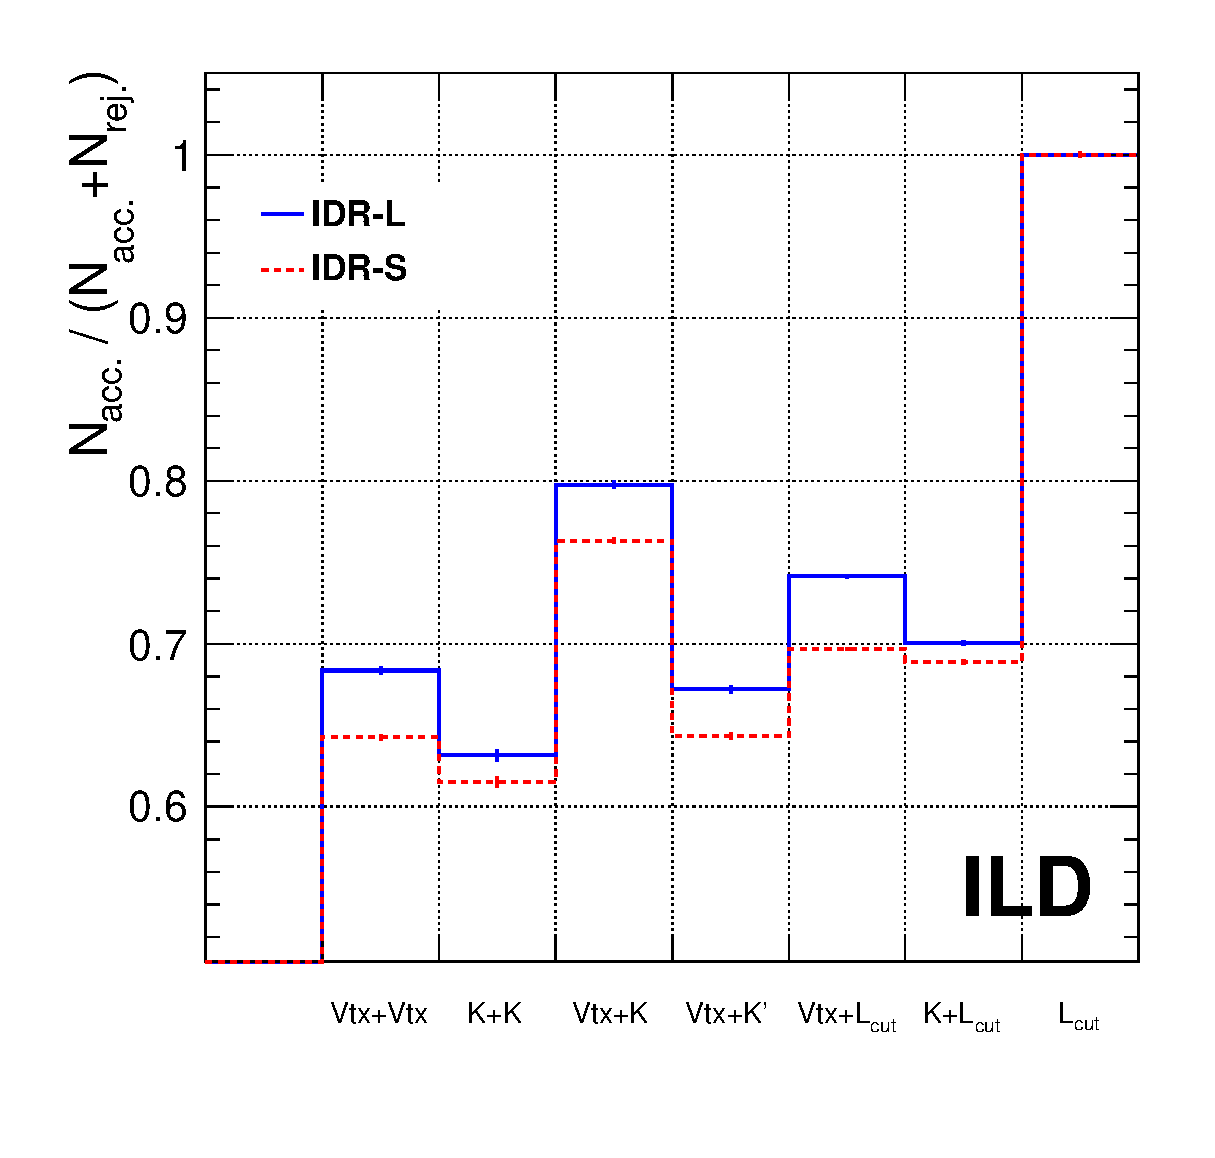
\includegraphics[width=0.5\textwidth]{figures_TTbar/p_value_num_l5_ele_mu.eps} & 
      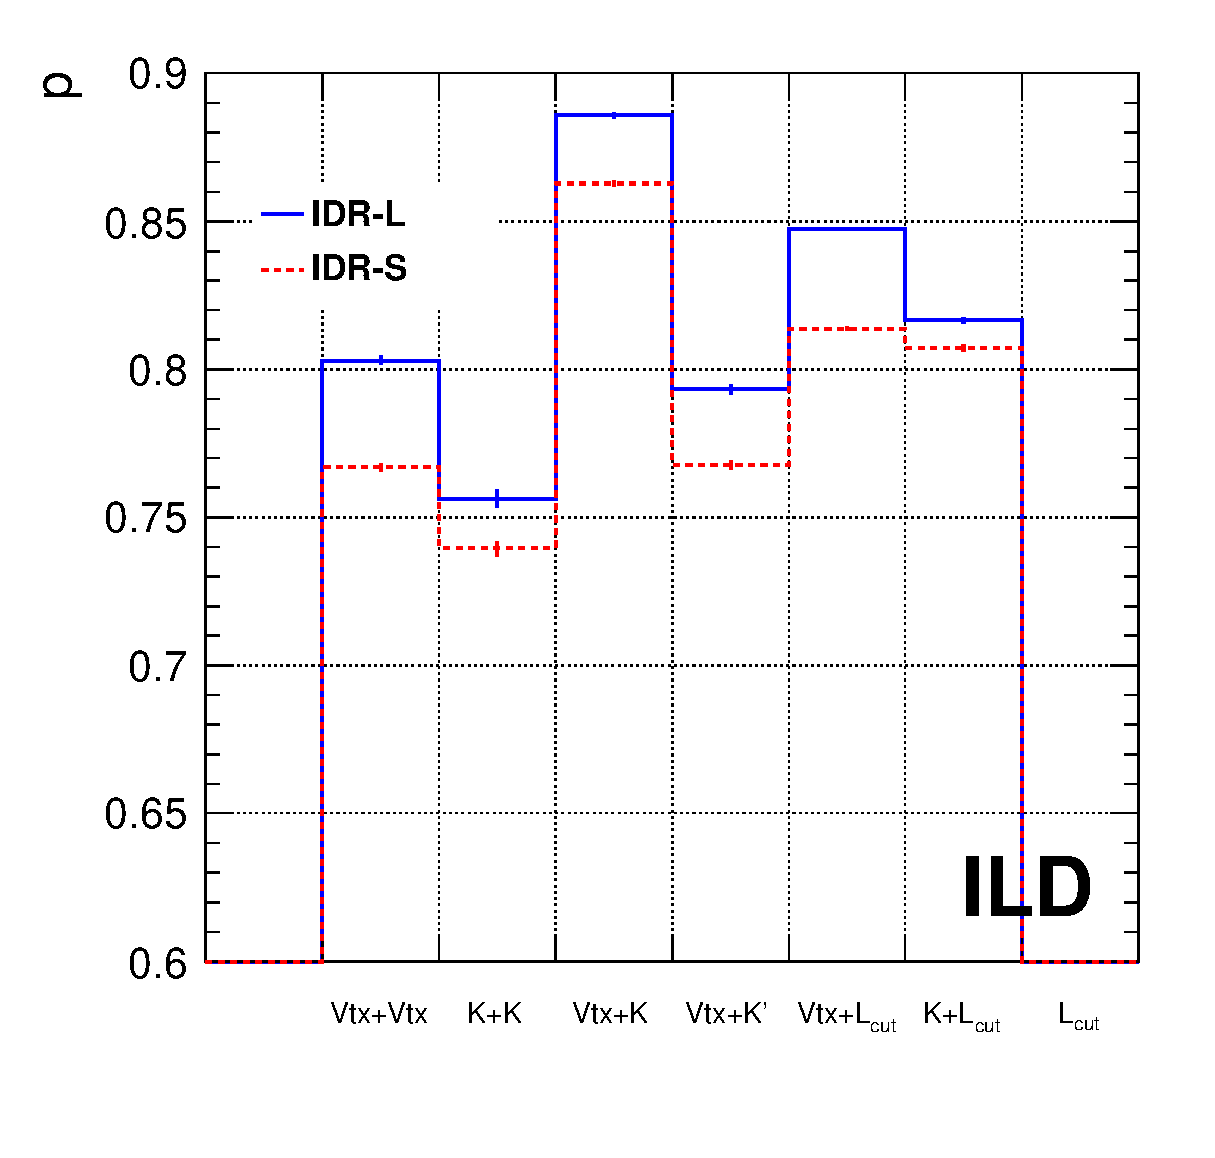
\includegraphics[width=0.5\textwidth]{figures_TTbar/p_value_l5_ele_mu.eps}
    \end{tabular}
    \caption{Calculated probability plots for $t\bar{t}$ events. Left plot shows the result of $N_{acc.} / (N_{acc.} + N_{rej.})$ and right plot shows the p values with different charge configurations.}
    \label{fig_eff_purity}
  \end{figure}

Table~\ref{tab:tt-eff} shows the overall selection efficiencies and the generated and reconstructed value of the forward-backward asymmetry $A_{FB}$ as an estimator for the quality of the reconstruction.

\begin{table}[h!]
    \parbox{.45\linewidth}{
    \centering
    \begin{tabular}{ccc}
      \hline
      \hline
      	Afb gen				&	0.328685		&	N: 1812768	\\
      	Afb reco			&	0.341900		&	N: 277435		\\
      	Final efficiency	&	30.609\%		&	\\			
      \hline
      \hline
    \end{tabular}
    \caption{l5 final efficiency and $A_{fb}$}
    }
    \hfill
    \parbox{.45\linewidth}{
    \centering
    \begin{tabular}{ccc}
      \hline
      \hline
        Afb gen				&	0.328848		&	N: 1866364	\\
      	Afb reco			&	0.340474		&	N: 284183		\\
      	Final efficiency	&	30.4531\%	&						\\	
      \hline
      \hline
  \end{tabular}
  \caption{s5 final efficiency and $A_{fb}$}
  \label{tab:tt-eff}
  }
  
  \end{table}

  \begin{table}[t]
    \begin{center}\renewcommand{\arraystretch}{1.6}
      \begin{tabular}{l|l|l} 
      \multicolumn{3}{c}{$e_{L}^{-}e_{R}^{+}\rightarrow t\bar{t}$ at 500 GeV }\\
        \hline
        \hline
         															& IDR-L & IDR-S\\
        \hline
        Isolated Lepton   									& 92.1\% & 92.1\% \\
        $btag_{1} > 0.8$ or $btag_{2} > 0.3$    	& 81.2\% & 81.1\% \\
        Thrust $< 0.9$   									& 81.2\% & 81.1\% \\
        Hadronic mass										& 78.2\% & 78.2\% \\
        Reconstructed $m_W$ and $m_t$			& 73.4\% & 73.4\% \\
        \hline
        \hline     
      \end{tabular}
   \end{center}
   \caption{Event selection efficiencies after each preselection criteria presented. Note that this does not concerns any background effects.}
   \label{table_precut_eff}
  \end{table}


%\end{itemize}




%\subsection{Limits of $ee\rightarrow bb$ at 500\,GeV}

%\begin{itemize}
%\item Here I wanted to point out why the bb at 500 GeV is more involved than at 250 GeV but given the results shown today by Adrian this is maybe less of an issue.
%\end{itemize}

%|||||||||||||||||||Interaction zone|||||||||||||||||||||||

\section{Results}
 
Figure~\ref{results_bb} shows the polar angle spectrum after the application of Eq.~\ref{eq:pq-meth} for the $e_{L}^{-}e_{R}^{+}\rightarrow b\bar{b}$. Large and small detector agree within statistical uncertainties. It seems however that there is larger migration for the small detector.  

 \begin{figure}[h!]
\centering
  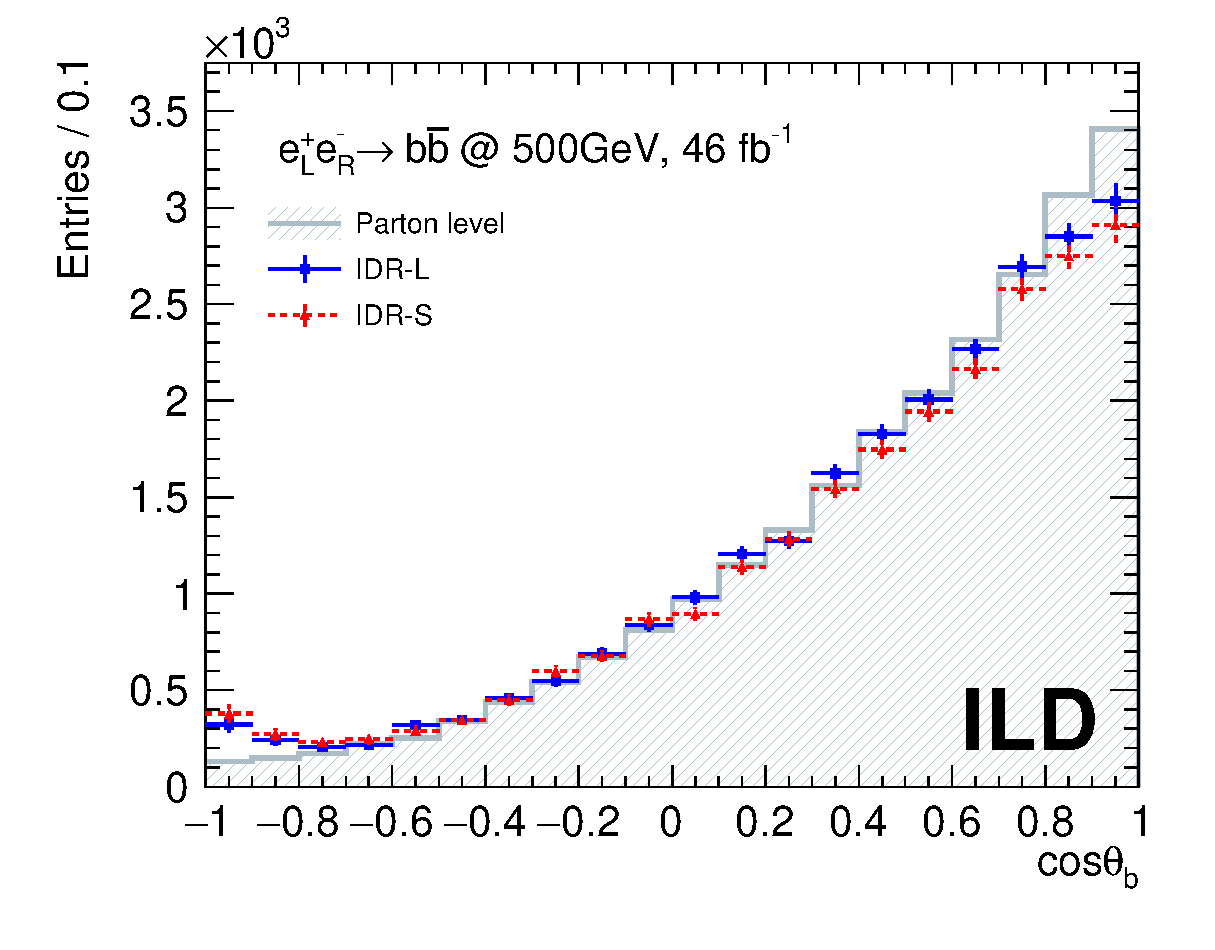
\includegraphics[width=0.6\textwidth]{figures_BBbar/result2models_v2.eps} 
\caption{}
\label{results_bb}
\end{figure}


The left part of Fig.~\ref{fig:res-ttbar} shows the polar angle distribution of $t\bar{t}$ of the generated and reconstructed data for the large and the small detector models. The red dotted line shows the fitted result of the reconstructed events. The right part shows the polar angle distribution of the underlying b-quark. 

\begin{figure}
\centering
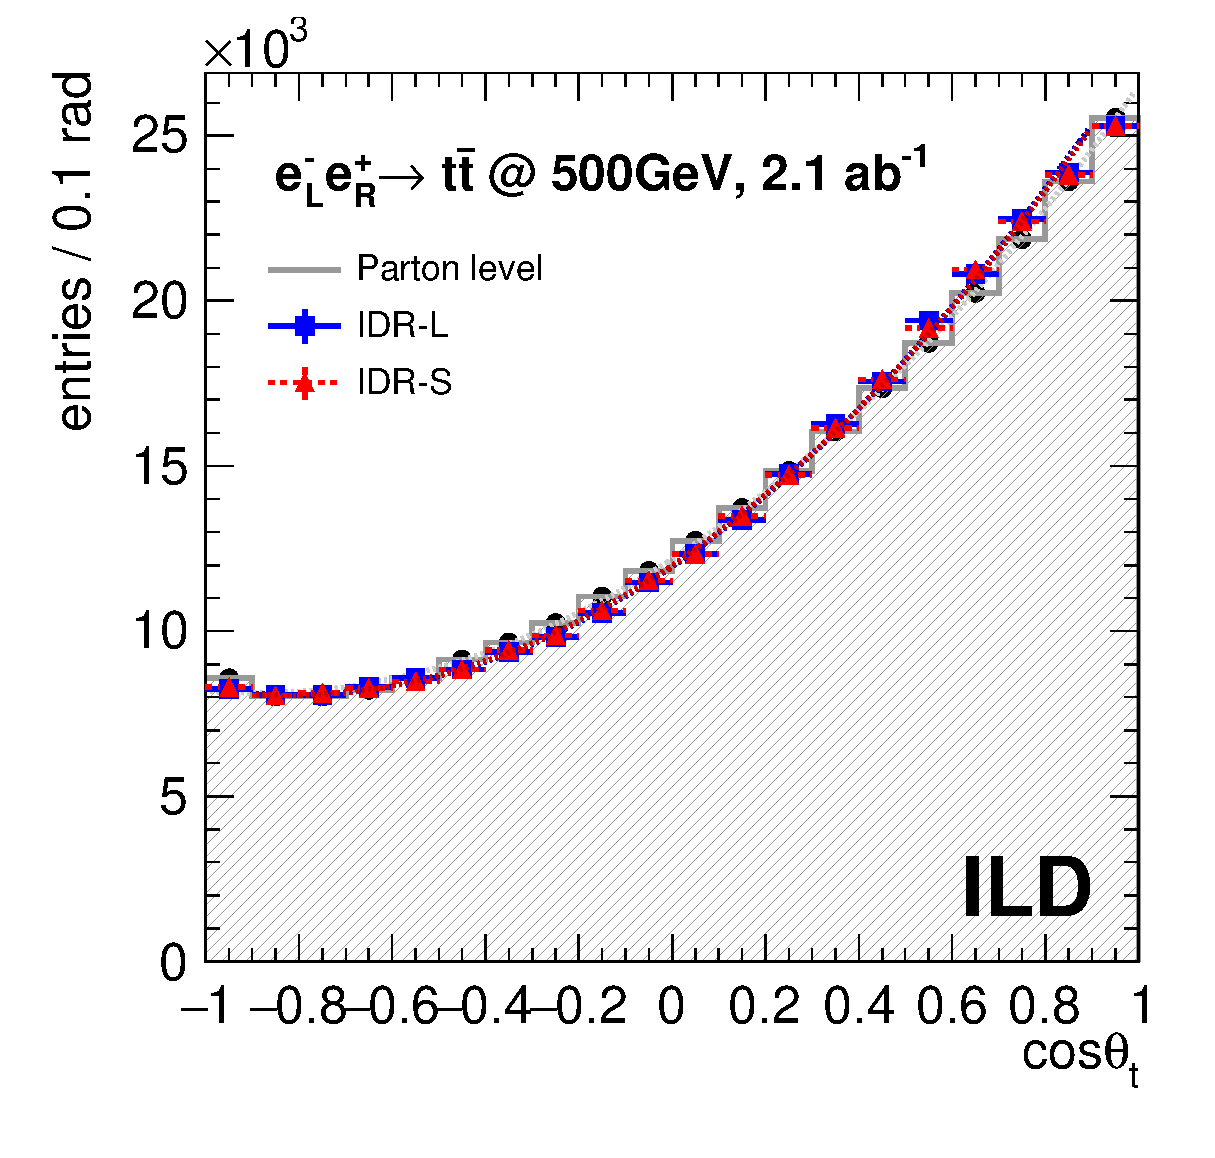
\includegraphics[width=0.45\textwidth]{figures_TTbar/results2models_t.eps}
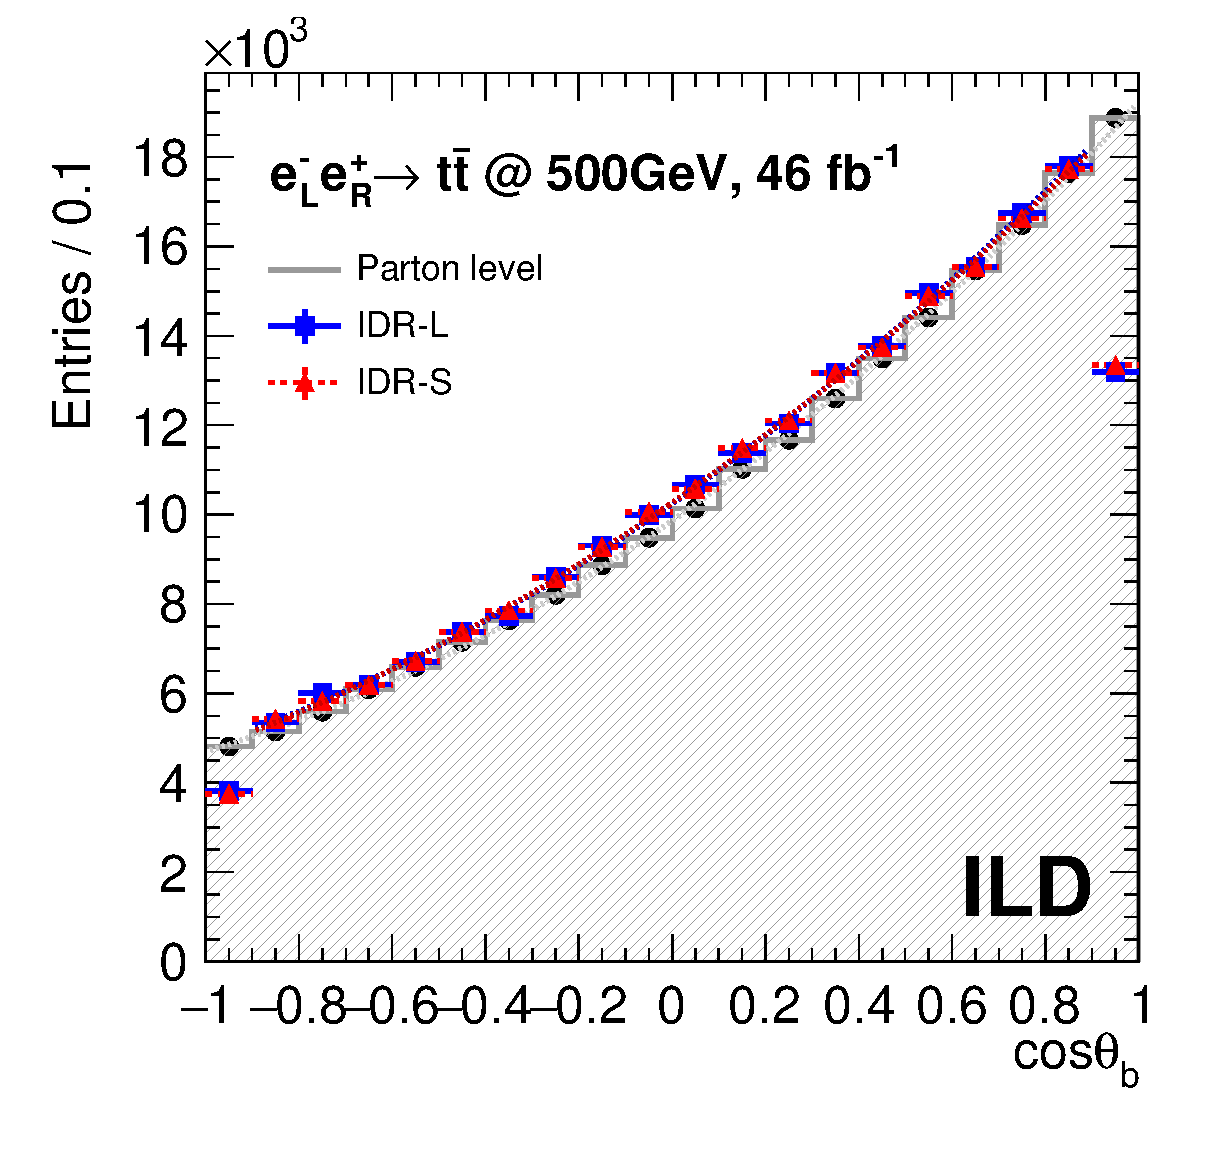
\includegraphics[width=0.45\textwidth]{figures_TTbar/results2models_b.eps}
\caption{\label{fig:res-ttbar} \sl \underline{Left:} Polar angle distribution for top quark.  will be on the same level. \underline{Right:}  Polar angle distribution for the b-quark that is issue of the top quark decay. The distributions for IDR-S is normalized to the one for IDR-L so that both histograms will be on the same level.. Distributions for IDR-S are normalised to the one for IDR-L so that both histograms}
\end{figure}

%\begin{itemize}
%\item Polar angle spectrum $ee\rightarrow bb$ (Large and small)
%\item $ee\rightarrow tt$  including underlying b polar angle spectrum (Large and small)
%\end{itemize}




%\begin{figure}[H]
%\centering
%\includegraphics[width=.50\linewidth]{new-ntracks-graph.pdf}
%\caption{\label{fig:fulltrackgraph} \sl The average number of secondary tracks $\left< N_{\mathrm{tracks}} \right>$ as a function of the beam energy. Other details follow those of Fig.~\ref{fig:irgraph}. 
%for data (black points with error shaded band) in comparison to the three simulation models, \qgsp\ (blue squares), \ftfp\ (green upward-pointing triangles) and \qbbc\ (red downward-pointing triangles).  Error bars represent statistical errors and the error band the systematic error from the correction for double $\uppi^-$ background.
%}
%\end{figure}

%|||||||||||||||||||||Hit distribution||||||||||||||||||||||


\section{Summary}

%The process $ee\rightarrow tt$ has been successfully ported from the `DBD world' to the `IDR World'. No major differences between short and large detectors. \\

SUMMARY FROM BBBAR ANALYSIS TO BE ADDED.

No significant differences were confirmed between s5 and l5 samples. For the $t\bar{t}$ studies, we see that the polar angle distribution is consistent with the Parton level result. At the edges of the polar angles, we do not see inefficiencies due to the detector geometry. Inefficiencies of at the edges of the detectors originates from inability to reconstruct b jets going to the forward region. For the top pair reconstruction, we can also rely on W informations thus not losing much efficiencies at the edges.

\section*{Acknowledgements}
%Tu peux faire ca avant la migration. 
%{\it [Data-set specific thanks to laboratories, technical staff, non-CALICE institutes providing equipment, ... --- not added now ---  ]}
%We gratefully acknowledge the DESY, CERN and FNAL managements for their support and hospitality, and their accelerator staff for the reliable and efficient beam operation.
%This work was supported 
%by the FWO, Belgium; 
%by the Natural Sciences and Engineering Research Council of Canada;
%by the Ministry of Education, Youth and Sports of the Czech Republic;
%by the European Union's Horizon 2020 Research and Innovation programme under Grant Agreement 654168; %% AIDA-2020
%by the European Commission within Framework Programme 7 Capacities, Grant Agreement 262025;  %% AIDA (not 2020)
%by the P2IO LabEx in the framework 'Investissements d'Avenir' managed by the French National Research Agency (ANR) under Grant Agreements ANR-10-LABX-0038 and ANR-11-IDEX-0003-01; 
%by the `Quarks and Leptons' Programme of CNRS/IN2P3 France;
%by the `Prestige/MSCA Programme;
%by the Alexander von Humboldt Stiftung (AvH), Germany;
%by the Bundesministerium f\"ur Bildung und Forschung (BMBF), Germany; 
%by the Deutsche Forschungsgemeinschaft (DFG), Germany; 
%by the Helmholtz-Gemeinschaft (HGF), Germany; 
%by the I-CORE Program of the Planning and Budgeting Committee, Israel;
%by the Nella and Leon Benoziyo Center for High Energy Physics, Israel;
%by the Israeli Science Foundation, Israel;
%by the National Research Foundation of Korea;
%by the Korea-EU cooperation programme of National Research Foundation of Korea, Grant Agreement 2014K1A3A7A03075053; 
%by the Netherlands Organisation for Scientific Research (NWO);
%by the Science and Technology Facilities Council, UK;
%by the Nuclear Physics, Particle Physics, Astrophysics and Cosmology Initiative, a Laboratory Directed Research and Development program at the Pacific Northwest National Laboratory, USA.
%{\it [add your funding agency here, grant numbers only if absolutely required]}.

%In conclusion, there is no preference for {\sc Geant4} physics lists as none of the two models, used in the analysis, describe the data in high detail. 
%-------------------------------------------------------------------
%-------------------------BIBLIOGRAPHY------------------------------
%-------------------------------------------------------------------
%\begin{thebibliography}{100} 
%\bibitem{bib:Calorimetry} J. C. Brient, H. Videau,\emph{ The calorimetry at the future $e^+e^-$ linear collider}, in: Proceedings of the APS / DPF / DPB Summer Study on the Future of Particle Physics (Snowmass 2001), 2001,arXiv:hep-ex/0202004v1.
%\bibitem{bib:ecal} The CALICE collaboration, \emph{Design and electronics commissioning of the physics prototype of a Si-W electromagnetic calorimeter for the International Linear Collider}, J. Instrum. 3 (2008) P08001, arXiv:0805.4833v1 [physics.ins-det]
%\bibitem{bib:Naomi} The CALICE Collaboration,  \emph{Testing Hadronic Interaction Models using a Highly Granular Silicon-Tungsten Calorimeter}, Nucl. Instrum. Meth. A Volume 794, Pages 240–254, arXiv:1411.7215v2 [physics.ins-det]
%\bibitem{bib:2010_CALICE_2} The CALICE Collaboration, C. Adloff, et al., \emph{Construction and Commissioning  of the CALICE Analog Hadron Calorimeter Prototype}, J. Instrum.~(5)  (2010) P05004, arXiv:1003.2662v1 [physics.ins-det].
%\bibitem{bib:2012_CALICE} The CALICE Collaboration, C. Adloff, et al., \emph{Construction and performance of a silicon photomultiplier/extruded scintillator tail-catcher and muon-tracker}, J. Instrum. (7) (2012) P04015, arXiv:1201.1653 [physics.ins-det].
%\bibitem{bib:G4pl} The {\sc Geant}4 Collaboration, \emph{Reference Physics Lists}, \url{http://Geant4.cern.ch/support/proc_mod_catalog/physics\_lists/referencePL.shtml}
%\bibitem{bib:HLi} \emph{Higgs Recoil Mass and Cross-Section Analysis at ILC And Calibration of the CALICE SiW ECAL Prototype}, Ph.D. thesis, Universit\'e Paris Sud   - Paris XI (2012).
%\bibitem{bib:2012_Doublet} P.Doublet, \emph{Hadrons dans un calorim\`etre \'electromagn\'etique   silicium-tungst\`ene hautement granulaire -- Production du quark top \'a   l'International Linear Collider}, Ph.D. thesis, Universit\'e Paris Sud   - Paris XI (2012).
%\end{thebibliography}
\section*{References}
\begin{footnotesize}
%
%\bibliographystyle{utphys_mod}
%\bibliography{had-pap}
%
%\bibliographystyle{hep}

%\renewcommand\refname{References}
%\end{thebibliography}
\end{footnotesize}


%The following plots in Fig. \ref{fig:rtotexample} and \ref{fig:rtotalrgraph} allow to establish a connection between Ref. \cite{bib:Naomi} and the present study. Regarding the difference in units of measurement and different selection by interaction layer, the Fig. \ref{fig:rtotalrgraph} is similar to its analogue in Ref. \cite{bib:Naomi}.
%\begin{figure}[H]
%\centering
%\begin{subfigure}{0.5\textwidth}
%\centering
%\includegraphics[width=.90\linewidth]{stdselection/r-total-2.pdf}
%\caption{\label{fig:rtot2} 2\,GeV primary particle.}
%\end{subfigure}% 
%\begin{subfigure}{0.5\textwidth}
%\centering
%\includegraphics[width=.90\linewidth]{stdselection/r-total-10.pdf}
%\caption{\label{fig:rtot10} 10\,GeV primary particle.}
%\end{subfigure}
%\caption{\label{fig:rtotexample} A comparison of mean radius of event hits between Monte Carlo samples and data with 2 (left) and 10 (right) GeV beam energy. The histograms are normalized to unity in order to compare samples with different event number. Error bars on the plot represent statistical uncertainties only.}
%\end{figure}

%\begin{figure}[H]
%\centering
%\includegraphics[width=0.5\textwidth]{stdselection/r-total-graph.pdf}
%\caption{\label{fig:rtotalrgraph} A mean radius of hits in the \ecal\ for data and various Monte Carlo physics lists as a function of beam energy (2\,GeV to 10\,GeV). Error regions on the graph represent statistical uncertainties only.}
%\end{figure}

%\begin{figure}[H]
%\centering
%\includegraphics[width=0.5\textwidth]{stdselection/combination.pdf}
%\caption{\label{fig:epsilondatasys} Mean number of tracks found by the \tfa\ with different \ep\ values for 2, 4, 6, 8 and 10\,GeV beam energy of the \qgsp\ simulation and data. The difference between data and corresponding simulation curves is caused by an underestimation of number of clusters by the physics list model. The saturation value of $<N_{tracks}>$ is gradually increasing with the beam energy. }
%\end{figure}

%\clearpage

%%%%%%%%%%%%%% 

%\section*{Analysis of $e^+e^-\rightarrow t\bar{t}$}

%\begin{itemize}

%\item Settings
%  \begin{itemize}
%  \item ILCSoft v02-00-02
%  \item Used yyxylv and yyxyev events (eliminated isolated tau)
%  \item Polarization of eLpR is used.
%  \end{itemize}
  
%\item Polar angle distribution of $t\bar{t}$
%  \begin{itemize}
%  \item Full statistic polar angle
%  \item Polar angle distribution of $t\bar{t}$ of the generated and reconstructed data. Red dotted line shows the fitted result of the reconstructed events.
%  \item $t\bar{t}$ polar angle for large (l5) and small (s5) models. (Figure.~\ref{compare})
      
%  \begin{figure}[h!]
%    \centering
%    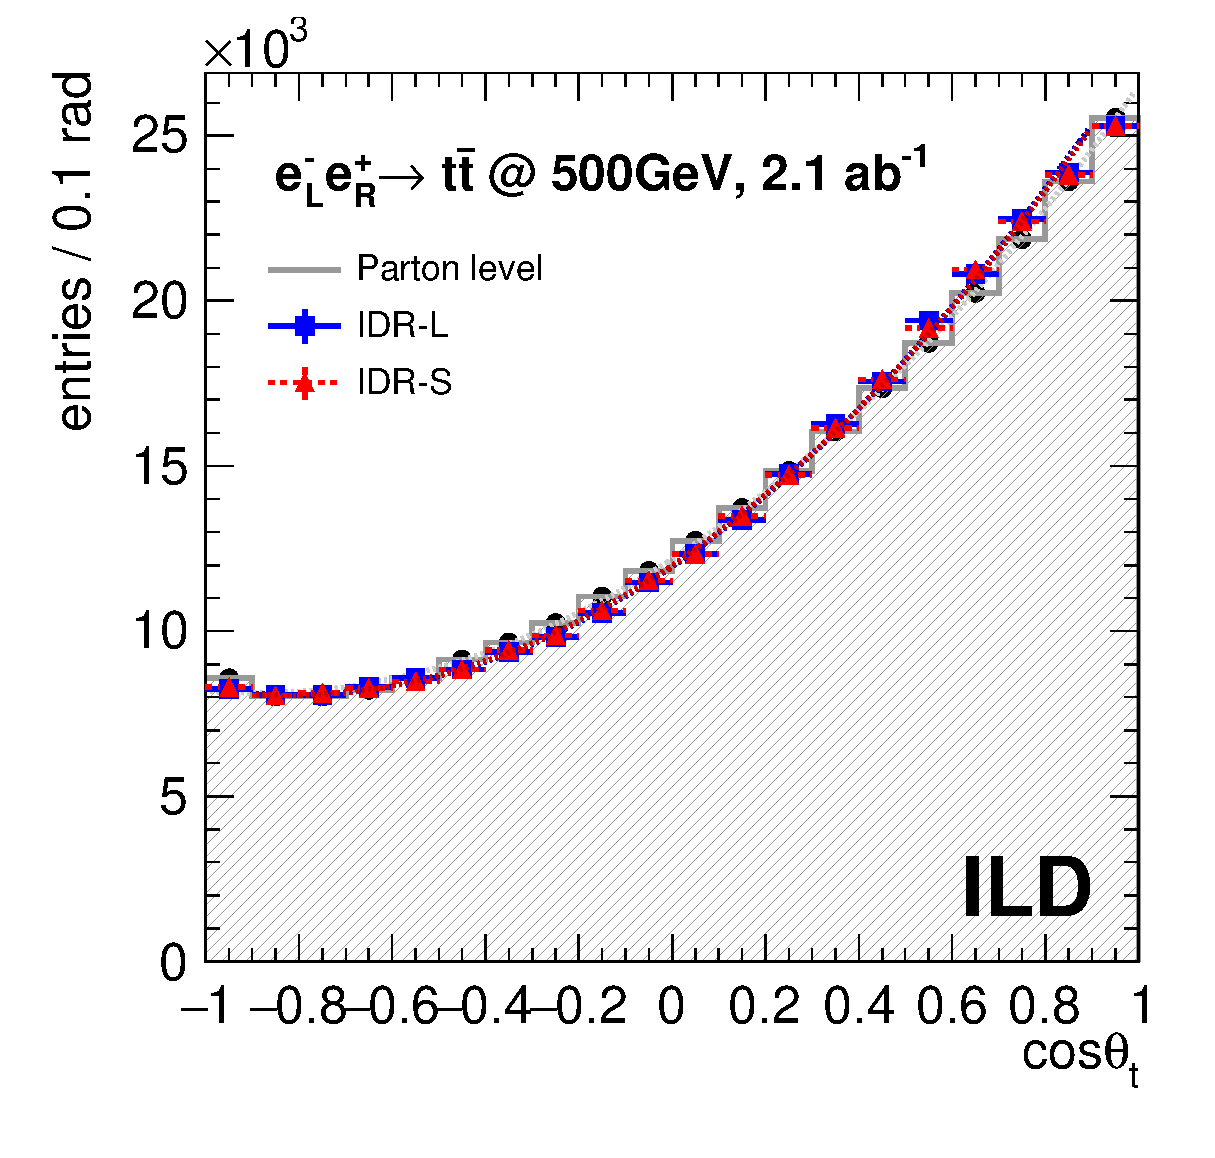
\includegraphics[width=0.5\textwidth]{figures_TTbar/results2models_t.eps} 
%    \caption{Polar angle distribution for top quark. Distributions for IDR-S is normalized to the one for IDR-L so that both histograms will be on the same level. }
%    \label{compare}
%  \end{figure}

%    \item Final efficiencies
    
    
 % \item No significant differences were confirmed between s5 and l5 samples. For the $t\bar{t}$ studies, we see that the polar angle distribution is consistent with the Parton level result. At the edges of the polar angles, we do not see inefficiencies due to the detector geometry. Inefficiencies of at the edges of the detectors originates from inability to reconstruct b jets going to the forward region. For the top pair reconstruction, we can also rely on W informations thus not losing much efficiencies at the edges.



%\break

  

%\end{itemize}

  
%  \item Polar angle distribution of $b\bar{b}$
%  \begin{itemize}
%  \item Full statistic polar angle
%  \item We could put each figures side by side for comparison. For example, we can put $t\bar{t}$ and $b\bar{b}$ plots side by side with same detector model.
%  \item $b\bar{b}$ polar angle for large (l5) and small (s5) models (Figure.~\ref{compare_b})
  
%    \begin{figure}[h!]
%      \centering
%        \begin{tabular}{ll}
%          \includegraphics[width=0.5\textwidth]{figures_TTbar/b_polar_l5_ele_mu.eps} & 
%          \includegraphics[width=0.5\textwidth]{figures_TTbar/b_polar_s5_ele_mu.eps}
%        \end{tabular}
%        \caption{Left is l5 and right is s5}
%        \label{fig_polar_ttbar}
%    \end{figure}

%     \begin{figure}[h!]
%        \centering
%        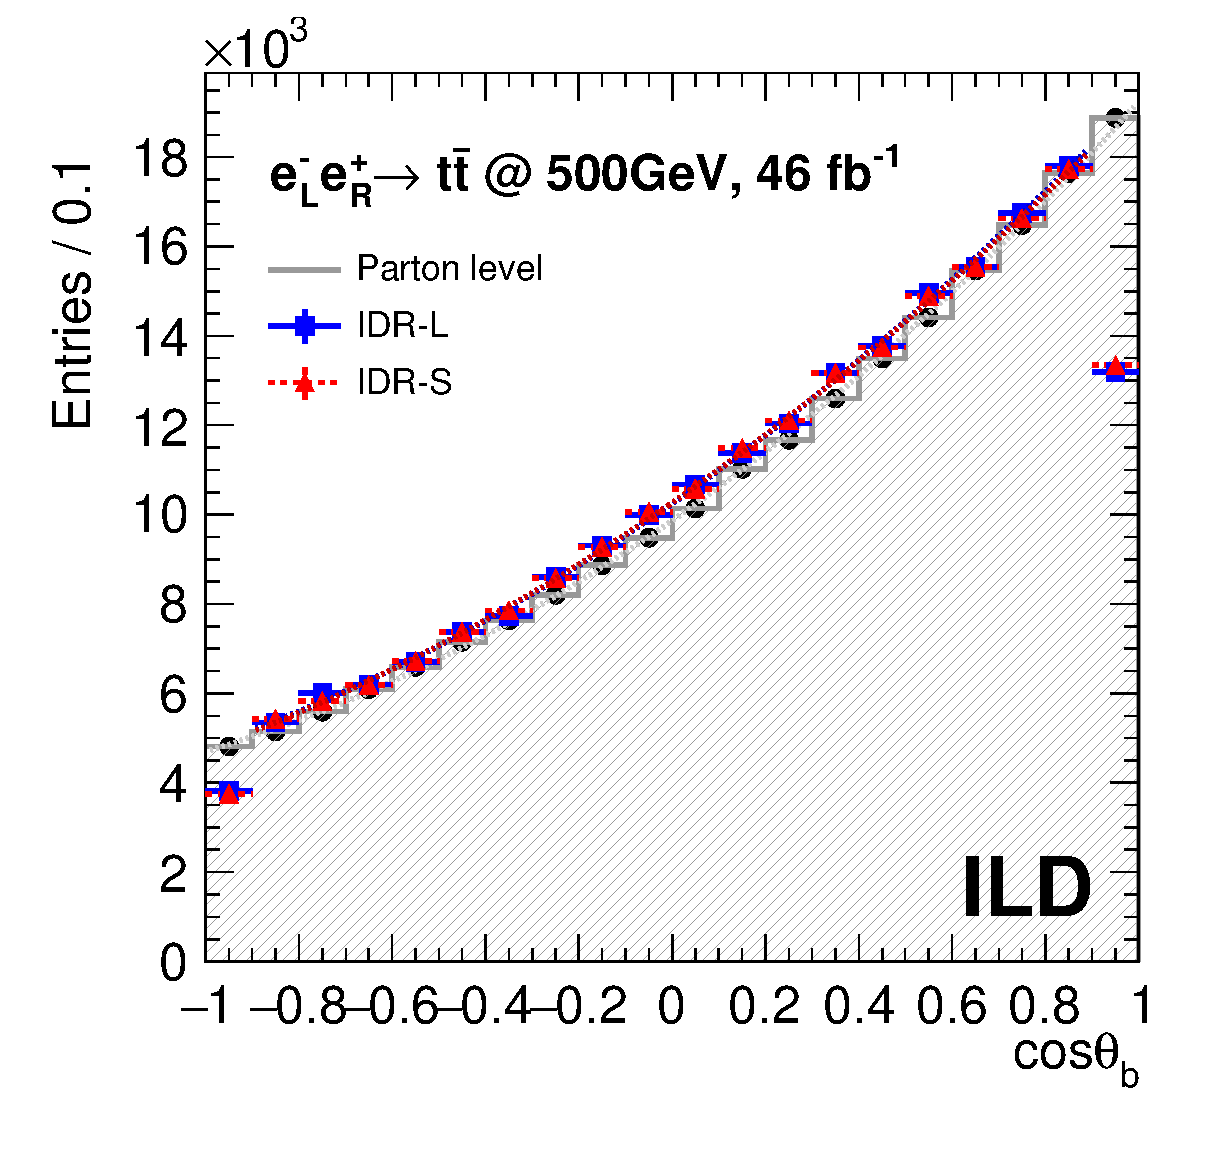
\includegraphics[width=0.5\textwidth]{figures_TTbar/results2models_b.eps} 
%        \caption{Hadronic polar angle distribution. Distributions for IDR-S is normalized to the one for IDR-L so that both histograms will be on the same level.}
%        \label{compare_b}
%    \end{figure}

  
%  \end{itemize}
  
  
%  \break
  

  \section*{Appendix}
      
    \begin{figure}[h!]
      \centering
        \begin{tabular}{ll}
          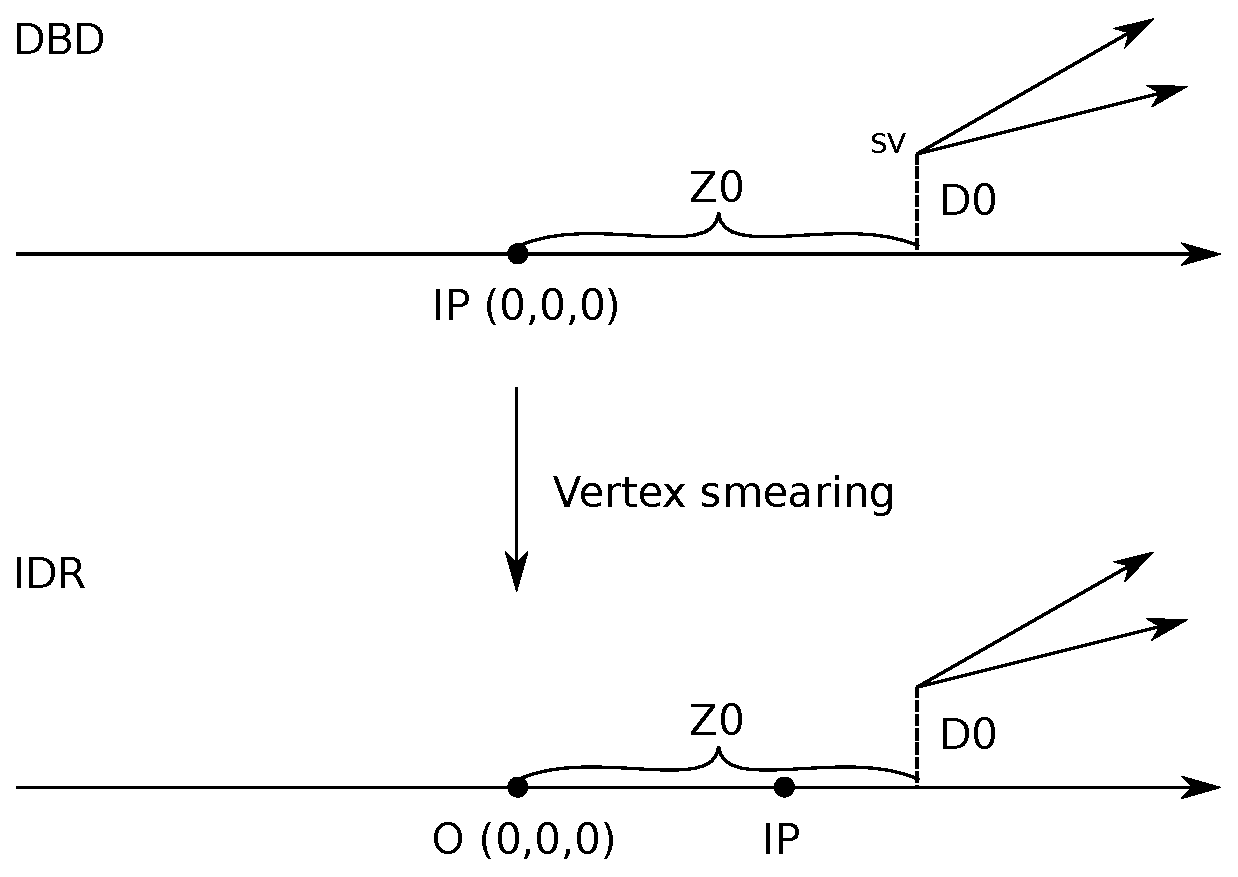
\includegraphics[width=0.5\textwidth]{figures_Methods/drawing.eps} & 
          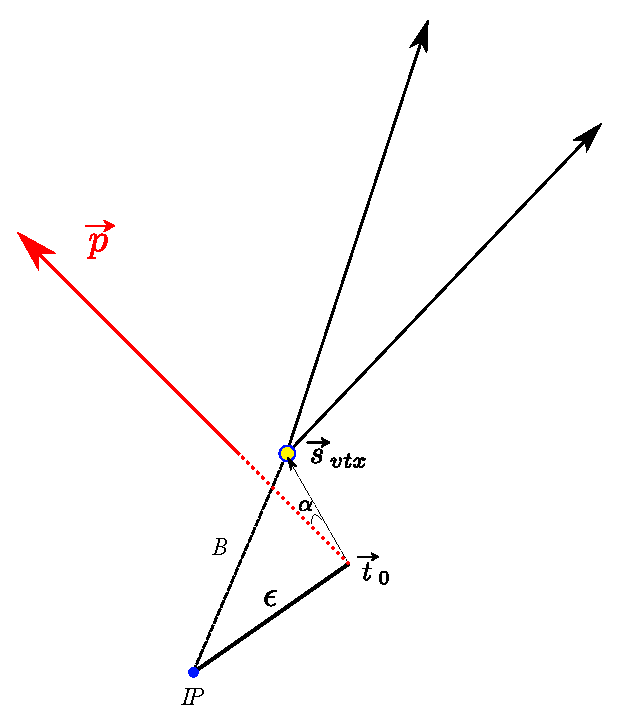
\includegraphics[width=0.5\textwidth]{figures_Methods/vertex_recovery.eps}
        \end{tabular}
        \caption{Left is }
        \label{fig_vtx_restore_schematics}
    \end{figure}
          
  
%\end{itemize}

\end{document}
